% ============================================================
%  Chapter 10: Delivering Food
%  Nature Inspired Optimisation for Delivery Problems (2022)
%  Self-contained Beamer slides — reader-friendly lecture notes
% ============================================================
\documentclass[aspectratio=169,10pt]{beamer}

\usetheme{Madrid}
\usecolortheme{seahorse}

\usepackage{amsmath,amssymb}
\usepackage{listings}
\usepackage{booktabs}
\usepackage{array}
\usepackage{xcolor}
\usepackage{graphicx}
\usepackage{hyperref}
\usepackage{microtype}

\graphicspath{{figures/}}

% ── listings style ────────────────────────────────────────────
\lstset{
  language=Java,
  basicstyle=\ttfamily\scriptsize,
  numbers=left,
  numberstyle=\tiny\color{gray},
  frame=single,
  backgroundcolor=\color{gray!7},
  keywordstyle=\color{blue!70!black}\bfseries,
  commentstyle=\color{green!50!black}\itshape,
  stringstyle=\color{red!60!black},
  breaklines=true,
  showstringspaces=false,
  tabsize=2,
}

\lstdefinestyle{python}{
  language=Python,
  basicstyle=\ttfamily\scriptsize,
  numbers=left,
  numberstyle=\tiny\color{gray},
  frame=single,
  backgroundcolor=\color{gray!7},
  keywordstyle=\color{blue!70!black}\bfseries,
  commentstyle=\color{green!50!black}\itshape,
  stringstyle=\color{red!60!black},
  breaklines=true,
  showstringspaces=false,
  tabsize=2,
}

% ── footline ──────────────────────────────────────────────────
\setbeamertemplate{footline}[frame number]
\setbeamertemplate{navigation symbols}{}

% ── title page ────────────────────────────────────────────────
\title[Ch.\,10: Delivering Food]{Chapter 10: Delivering Food}
\subtitle{Nature Inspired Optimisation for Delivery Problems (2022)}
\author{}
\date{}

% ============================================================
\begin{document}
% ============================================================

\begin{frame}
  \titlepage
\end{frame}

% ── Table of Contents ─────────────────────────────────────────
\begin{frame}{Chapter Overview}
  \tableofcontents
\end{frame}

% ============================================================
\section{10.1 Introduction}
% ============================================================

\begin{frame}[allowframebreaks]{10.1 Introduction: Food Delivery in the Real World}

  The COVID-19 pandemic fundamentally changed how food is distributed
  in many countries.  Home delivery of food — from restaurants,
  supermarkets, and meal-kit companies — became a mainstream service
  almost overnight, requiring small businesses and community organisations
  to plan delivery routes that had previously been handled informally or
  not at all.

  \begin{block}{The Core Problem}
    A vehicle starts from a \textbf{depot}, must visit a set of
    customers, deliver food to each one within certain time and capacity
    constraints, and then return to the depot.  The goal is to minimise
    the total effort (distance or time) while satisfying all constraints.
    This is a specialised form of the \textbf{Vehicle Routing Problem
    (VRP)}.
  \end{block}

  Unlike parcel delivery, food delivery has several characteristics that
  make it particularly challenging in practice:

  \medskip
  \textbf{Time-sensitive goods.}
  Food quality degrades if it is not delivered within a reasonable time.
  This imposes a maximum round-trip time on each delivery vehicle
  (for example, 500 minutes per round in the experimental instance used
  in this chapter).

  \medskip
  \textbf{Variable demand.}
  Different customers may order different quantities (measured in units
  such as ``bag counts'').  The vehicle has a finite \emph{capacity}
  (maximum units it can carry), so it may need to make multiple rounds
  if the total demand exceeds that capacity.

  \medskip
  \textbf{Small, inexperienced operators.}
  The organisations deploying this software (such as volunteer food banks
  or small restaurants) may lack logistics expertise.  The optimisation
  must be packaged as a simple-to-use application — not a research
  prototype.

  \medskip
  \textbf{A ``bag'' as the unit of delivery.}
  The problem treats demand in discrete units called \emph{bags}.
  Each customer requires a certain number of bags, and a vehicle can
  carry at most $Q$ (Q) bags per round.  Throughout the book the quantity
  $Q$ denotes \emph{vehicle capacity}: the maximum load (in bags) that
  can be loaded onto the vehicle at any one time.

  \framebreak

  \begin{figure}
    \centering
    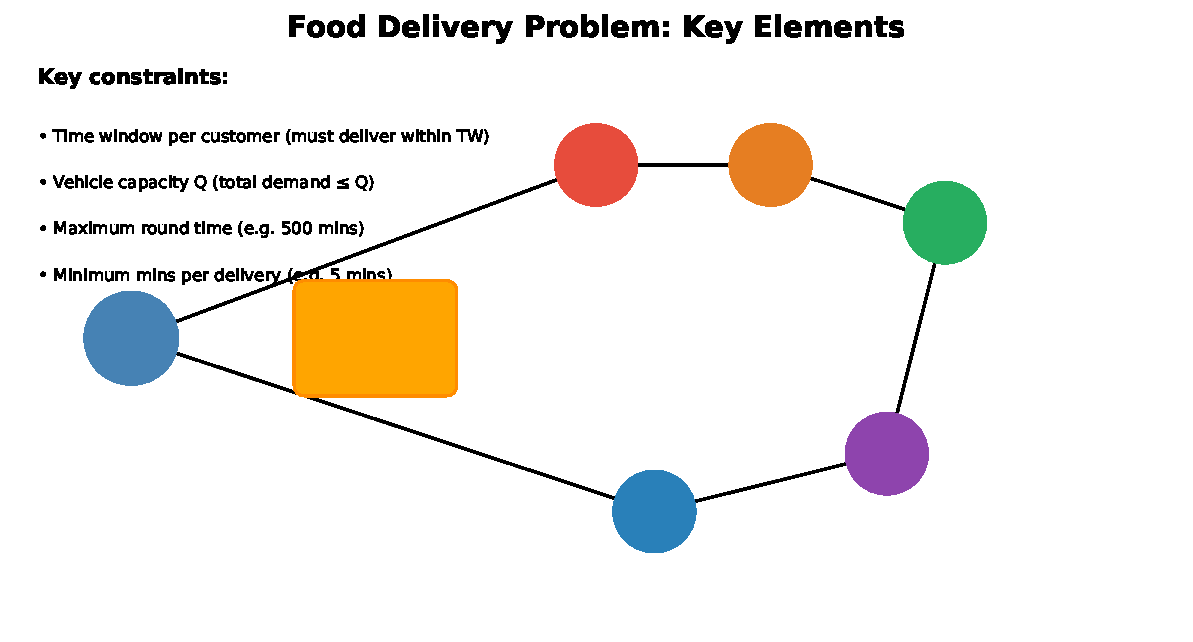
\includegraphics[width=0.80\textwidth]{fig_food_delivery_context.pdf}
    \caption{Key elements of the food delivery problem.
             The vehicle leaves the Depot, visits customers A–E, and
             must return within the time limit.  Both capacity $Q$
             (total bags) and the maximum transit time constrain which
             solutions are feasible.}
  \end{figure}

  \begin{alertblock}{Key Insight: Why This Problem Is Hard}
    Even for a modest fleet with 20--100 delivery stops, the number of
    possible orderings grows factorially.  Exhaustive enumeration is
    completely impractical, so we rely on \textbf{nature-inspired
    (evolutionary) algorithms} to search the solution space efficiently.
  \end{alertblock}

\end{frame}

% ============================================================
\section{10.2 Fitness}
% ============================================================

\begin{frame}[allowframebreaks]{10.2 Fitness: Choosing the Right Objective Function}

  The \emph{fitness function} (also called the \emph{objective
  function}) is the mathematical formula that scores each candidate
  solution.  A good fitness function does not merely measure \emph{what}
  the algorithm does — it guides \emph{how} the algorithm improves.
  Choosing the wrong fitness function can cause the algorithm to find
  technically correct but practically poor solutions.

  \framebreak

  \begin{block}{Candidate 1: Total Distance}
    The simplest approach is to sum the distance of every leg of the
    route:
    \[
      F_{\text{dist}} = \sum_{i=1}^{n} d_i
    \]
    where $d_i$ (``d sub i'') is the distance of the $i$-th leg and
    $n$ (n) is the total number of legs in the route
    (including the final return leg to the depot).
    The index $i$ runs from $1$ to $n$, so $\sum$ (Sigma, meaning
    ``sum over all legs'') adds up all $n$ distances.
  \end{block}

  \begin{block}{Notation}
    \begin{itemize}
      \item $d_i$ — distance (e.g.\ in kilometres or minutes) of leg
            number $i$ of the route.
      \item $n$ — total number of legs: for a route visiting $k$
            customers, $n = k + 1$ (the return leg counts too).
      \item $\sum_{i=1}^{n}$ — Sigma: ``add up the values
            $d_1, d_2, \ldots, d_n$ one by one''.
    \end{itemize}
  \end{block}

  \textbf{Why total distance is insufficient.}
  Consider a route visiting customers A, B, C, D, E in some order,
  where customers care about \emph{when} they are visited, not just
  whether they are visited.  A route that drives 10 km to the furthest
  customer first and then collects several nearby customers on the way
  back scores the same total distance as a route that delivers to
  nearby customers first — yet customers served late in the route must
  wait much longer.

  \framebreak

  \begin{block}{Candidate 2: Weighted Distance}
    The \textbf{weighted distance} (WD) assigns a weight to each leg
    equal to the number of customers who have \emph{not yet been
    served} at the start of that leg:
    \[
      WD = \sum_{i=1}^{n} d_i \times wc_i
    \]
    where $wc_i$ (``wc sub i'', standing for \emph{wait count}) is
    the number of remaining deliveries at the start of leg $i$.
  \end{block}

  \begin{block}{Notation}
    \begin{itemize}
      \item $d_i$ — distance of leg $i$ (same as before).
      \item $wc_i$ — ``wait count'' for leg $i$: the number of
            customers who have \textbf{not yet received} their delivery
            when the vehicle starts leg $i$.  For a route with $k$
            customers, $wc_1 = k$, $wc_2 = k-1$, \ldots, $wc_k = 1$,
            and the return leg $wc_{k+1} = 0$.
      \item $\sum_{i=1}^{n} d_i \times wc_i$ — sum of (distance of
            leg $i$) multiplied by (number of customers still waiting
            at the start of leg $i$).
    \end{itemize}
  \end{block}

  \begin{alertblock}{How to Read This Formula}
    Every metre travelled while customers are still waiting
    ``costs'' more than metres travelled after all deliveries are
    complete.  A long drive \emph{early} in the route is penalised
    heavily because many customers are waiting; a long return drive
    \emph{after} all deliveries are done has zero weight and costs
    nothing in WD terms.  Minimising WD therefore pushes the
    algorithm towards \textbf{making deliveries as early as possible
    in the route}.
  \end{alertblock}

  \framebreak

  \textbf{Worked Numerical Example.}
  Suppose we have a route Depot $\to$ A $\to$ B $\to$ C $\to$ D $\to$
  E $\to$ Depot with leg distances 2, 5, 6, 5, 3, 4 (total = 25).
  The wait counts are 5, 4, 3, 2, 1, 0 (decreasing by 1 after each
  delivery).

  \begin{exampleblock}{Worked Example: Computing WD}
    \begin{tabular}{lrrrrrrr}
      \toprule
      & Dep$\to$A & A$\to$B & B$\to$C & C$\to$D & D$\to$E
        & E$\to$Dep & Total \\
      \midrule
      Distance $d_i$ & 2 & 5 & 6 & 5 & 3 & 4 & 25 \\
      Wait count $wc_i$ & 6 & 5 & 4 & 3 & 2 & 1 & -- \\
      $d_i \times wc_i$ & 12 & 25 & 24 & 15 & 6 & 4 & \textbf{86} \\
      \bottomrule
    \end{tabular}

    \medskip
    The \textbf{simple distance} fitness is 25.
    The \textbf{weighted distance} fitness is 86.
    These two numbers measure very different things:
    WD = 86 captures the total ``waiting cost'' accumulated across
    all customers, rewarding routes that serve customers quickly.
    To minimise WD, the algorithm should place \emph{shorter} legs
    early in the route.
  \end{exampleblock}

  \begin{figure}
    \centering
    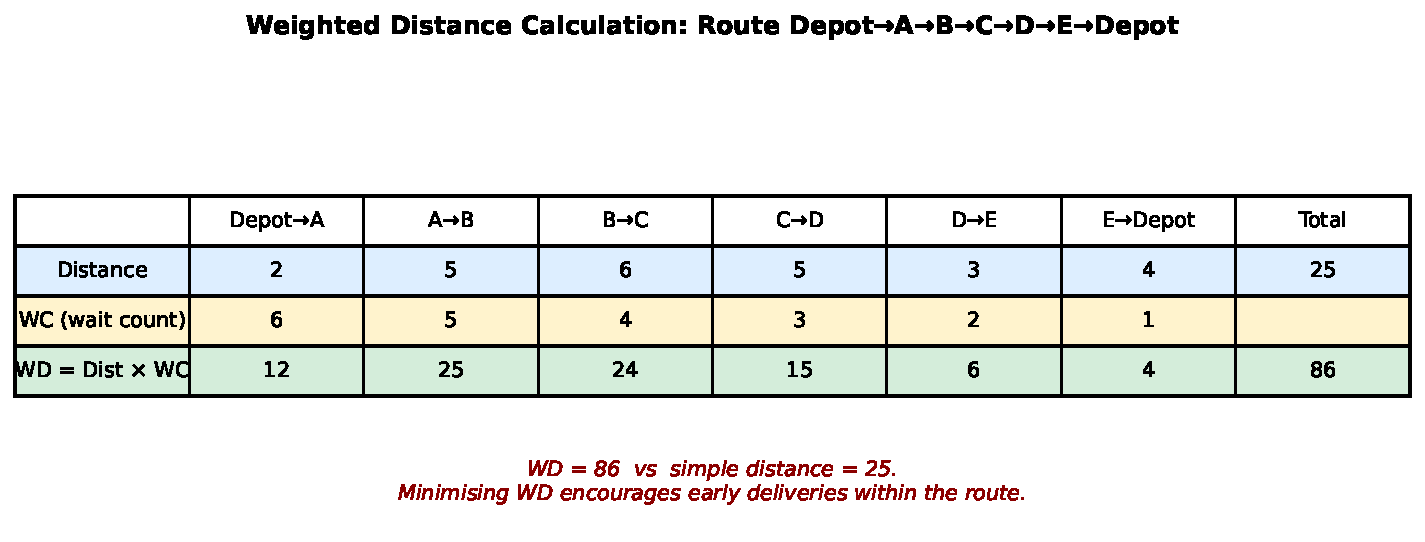
\includegraphics[width=0.78\textwidth]{fig_weighted_distance_table.pdf}
    \caption{Visual summary of the weighted-distance calculation.
             Each cell in the WD row is distance $\times$ wait count.
             The total WD (86) is much larger than total distance (25),
             reflecting the accumulated waiting cost.}
  \end{figure}

  \framebreak

  \begin{figure}
    \centering
    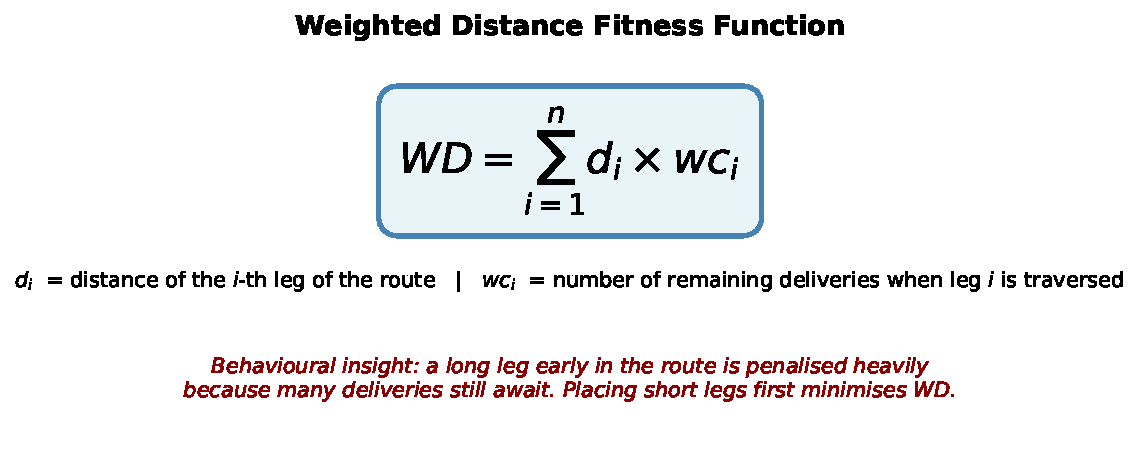
\includegraphics[width=0.65\textwidth]{fig_weighted_distance_formula.pdf}
    \caption{The weighted-distance formula.
             Long legs early in the route are penalised heavily because
             $wc_i$ is large; by the time all customers have been served,
             $wc_i = 0$ and any return leg is free.}
  \end{figure}

  \framebreak

  \textbf{Three route strategies and their WD values.}
  Given a set of customers, three natural strategies exist for ordering
  deliveries:

  \begin{itemize}
    \item \textbf{Route (a) — outward then return:}
      Visit customers from nearest to furthest, return directly.
      Simple distance is small, but WD may be large if the furthest
      customer is served very late.
    \item \textbf{Route (b) — furthest first:}
      Drive to the furthest point first, deliver on the way back.
      Some deliveries happen early; WD is lower.
    \item \textbf{Route (c) — mixed:}
      Make some deliveries on the outward journey and some on the
      return.  This can achieve a good balance, and feedback from
      real users of the system confirmed that this pattern was most
      expected.
  \end{itemize}

  When the \emph{time window} constraint is not tight, routes (b) and
  (c) are often equivalent in WD.  When the time constraint \emph{is}
  tight, the algorithm must find a feasible solution at all — any
  infeasible solution is penalised heavily.

  \begin{figure}
    \centering
    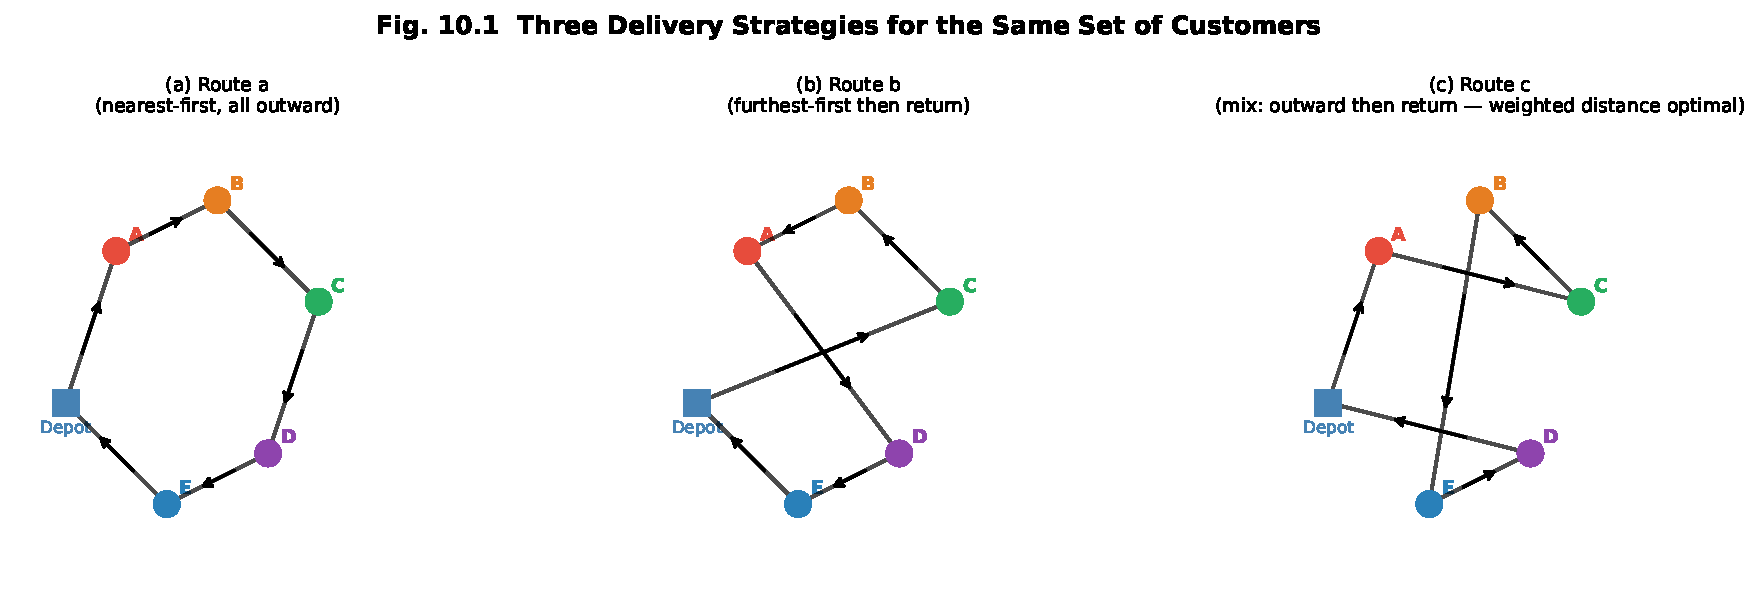
\includegraphics[width=0.92\textwidth]{fig_three_routes.pdf}
    \caption{Three candidate delivery strategies for the same customer
             set.  Route (a) delivers outward (nearest-first); route (b)
             delivers furthest-first; route (c) is a mixed approach.
             Minimising WD favours placing the shortest legs earliest,
             which often corresponds to route (b) or (c).}
  \end{figure}

  \framebreak

  \begin{figure}
    \centering
    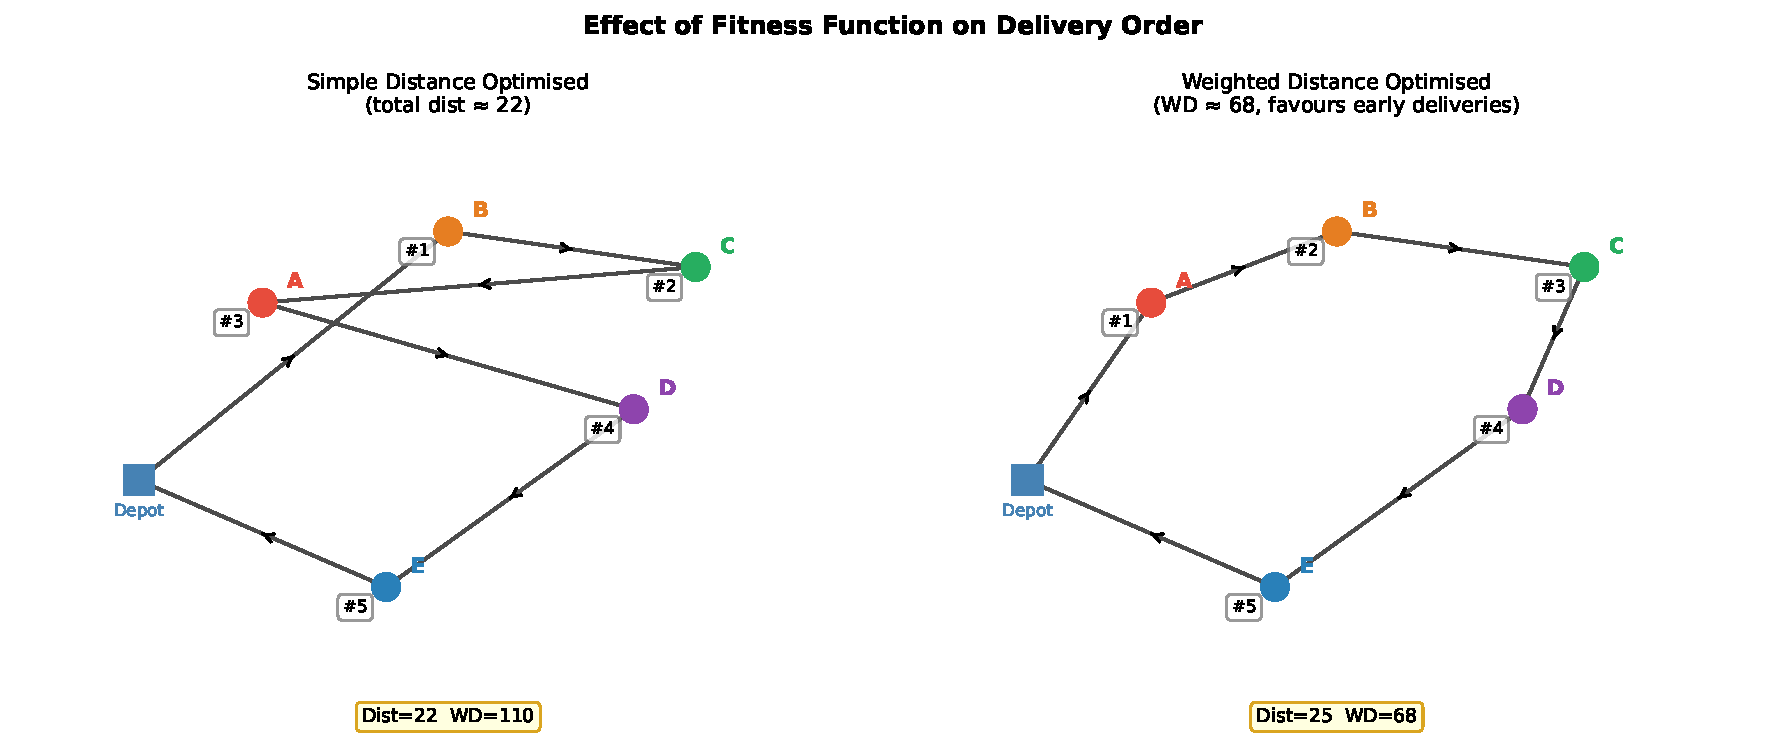
\includegraphics[width=0.80\textwidth]{fig_delivery_order_comparison.pdf}
    \caption{How the fitness function changes delivery order.
             \emph{Left:} optimising simple total distance may leave
             nearby customers until last.
             \emph{Right:} optimising weighted distance forces the
             algorithm to serve nearby customers first, reducing
             accumulated waiting.}
  \end{figure}

  \begin{alertblock}{Key Insight: Fitness Shapes Behaviour}
    The choice of fitness function is not a technical detail — it
    \textbf{determines what behaviour the algorithm is rewarded for}.
    Using total distance alone would produce routes that minimise
    mileage but may keep customers waiting for hours.  Weighted
    distance aligns the algorithm's objective with the actual goal:
    serve customers as promptly as possible.
  \end{alertblock}

\end{frame}

% ============================================================
\section{10.3 Implementation Issues}
% ============================================================

\begin{frame}[allowframebreaks]{10.3 Implementation Issues: Real-World Complications}

  Translating the mathematical model into a working software application
  requires careful engineering decisions that go beyond the algorithm
  itself.  This section describes the architecture of the demonstration
  application and the practical challenges encountered.

  \begin{block}{Three-Layer Architecture}
    The application is built in three clearly separated layers,
    following the software engineering principle of \emph{separation of
    concerns}:
    \begin{enumerate}
      \item \textbf{Imported base classes} — reusable components from
            earlier chapters: population management, route data
            structures, geospatial utilities, and file I/O.
      \item \textbf{Food-specific classes} — subclasses whose names
            begin with \texttt{Food}: \texttt{FoodPopulation},
            \texttt{FoodRoute}, \texttt{FoodEvaluator}.  These
            specialise the evaluation function and genetic operators
            for the food-delivery problem.
      \item \textbf{Application layer} — a single class called
            \texttt{FoodFacade}, implemented using the \emph{Facade}
            design pattern.  It exposes a clean, simple API to the
            calling application, hiding all optimisation details.
    \end{enumerate}
  \end{block}

  \begin{figure}
    \centering
    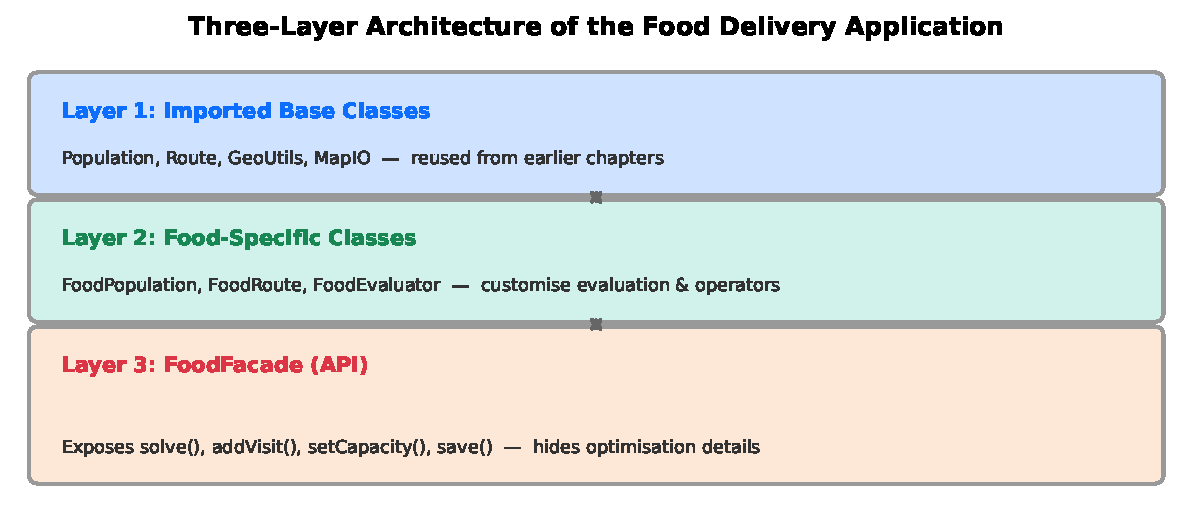
\includegraphics[width=0.80\textwidth]{fig_architecture_layers.pdf}
    \caption{The three-layer architecture.
             Layer 1 is reused from earlier chapters; Layer 2 extends
             it for food delivery; Layer 3 (the Facade) is the only
             component visible to the calling application.}
  \end{figure}

  \framebreak

  \begin{figure}
    \centering
    
\includegraphics[width=0.90\textwidth]{fig_class_diagram.pdf}
    \caption{Detailed class diagram showing the inheritance and usage
             relationships between the three layers.  Base classes
             (Layer 1, blue) are inherited or used by food-specific
             classes (Layer 2, green), which are in turn accessed only
             through \texttt{FoodFacade} (Layer 3, orange).}
  \end{figure}

  \framebreak

  \begin{block}{The Facade Design Pattern}
    The \emph{Facade pattern} (described by Erich Gamma et al.,
    1994, ``Design Patterns'') is a structural design pattern in which
    a single class provides a simplified interface to a complex
    subsystem.  By accessing the optimiser only through
    \texttt{FoodFacade}, the calling application is completely
    shielded from changes in algorithm parameters, geocoding
    libraries, or file-format details.  The optimisation algorithm
    can be upgraded without any change to the calling code.
  \end{block}

  \begin{exampleblock}{Why This Architecture Matters}
    The food-delivery solver could be embedded as a module within a
    larger system — for example, an e-commerce platform that handles
    online orders, stock control, and payment processing.
    The calling system simply invokes \texttt{FoodFacade.solve()} and
    receives the optimised routes; it never needs to know anything
    about evolutionary algorithms, mutation rates, or population sizes.
  \end{exampleblock}

  \framebreak

  \begin{block}{FoodFacade API (Table 10.1)}
    The following methods are exposed to application programmers:
  \end{block}

  \begin{center}
    \small
    \begin{tabular}{>{\ttfamily}lp{6.5cm}}
      \toprule
      \normalfont\textbf{Method Signature} & \textbf{Purpose} \\
      \midrule
      FoodFacade() & Constructor — creates a new solver instance \\
      solve() & Runs the optimiser and stores the best solution found \\
      addVisit(name, address, demand, order) & Registers one delivery stop with its address and bag count \\
      setStart(addr) & Sets the depot (start/end address) \\
      setReference(ref) & Labels this problem instance \\
      save(SaveTo) & Saves the solution (CONSOLE, KML, GPX, or CSV) \\
      setStartDateTime(dateTime) & Sets the departure time (dd/MM/yyyy HH:mm) \\
      setRoundMode(type) & Sets travel mode: ``car'', ``bike'', etc. \\
      setCapacity(cap) & Maximum bags the vehicle can carry per round \\
      setMinsDel(minsDel) & Minutes required per delivery stop \\
      setMaxMinsRound(maxMinsRound) & Maximum total time per round \\
      \bottomrule
    \end{tabular}
  \end{center}

  \medskip
  Notice that \emph{all details of the algorithm} — mutation rate,
  population size, number of generations — are hidden behind
  \texttt{solve()}.  The developer only specifies the problem
  (customers, capacity, time limit) and asks for a solution.

  \framebreak

  \begin{block}{Storing Algorithm Parameters}
    When the solver is bundled into a larger product, the developer
    cannot change source code to modify algorithm parameters.
    The application stores parameters such as mutation rate and
    population size in a \emph{configuration file} or \emph{properties
    file} (e.g.\ a Java \texttt{.properties} file).
    Figure 10.2 in the book shows a sample properties file.
    This approach allows non-programmer users — or system
    administrators — to tune algorithm behaviour without recompiling.
  \end{block}

  \begin{block}{Termination Strategy}
    Two complementary strategies control when the algorithm stops:
  \end{block}

  \begin{enumerate}
    \item \textbf{Stop and Resume.}
      A graphical user interface (GUI) presents ``Pause'' and
      ``Accept'' buttons alongside the current best solution.
      The user can pause the algorithm, examine the solution visually,
      then either press ``Accept'' (to take the current best result)
      or allow the algorithm to continue evolving.
      Restarting from a new random population is also possible,
      giving a fresh search for a fixed time budget.

    \item \textbf{Timeout.}
      A fixed evaluation budget (or wall-clock time limit) is set in
      the configuration.  The algorithm runs to the budget and then
      automatically returns the best solution found.  This guarantees
      that the user always receives an answer within a predictable time,
      which is essential for interactive applications and
      service-level agreements.
  \end{enumerate}

  The two strategies can be combined: a timeout guarantees an answer,
  while a ``Stop'' button allows the user to accept an intermediate
  result early if it already looks good.

  \begin{figure}
    \centering
    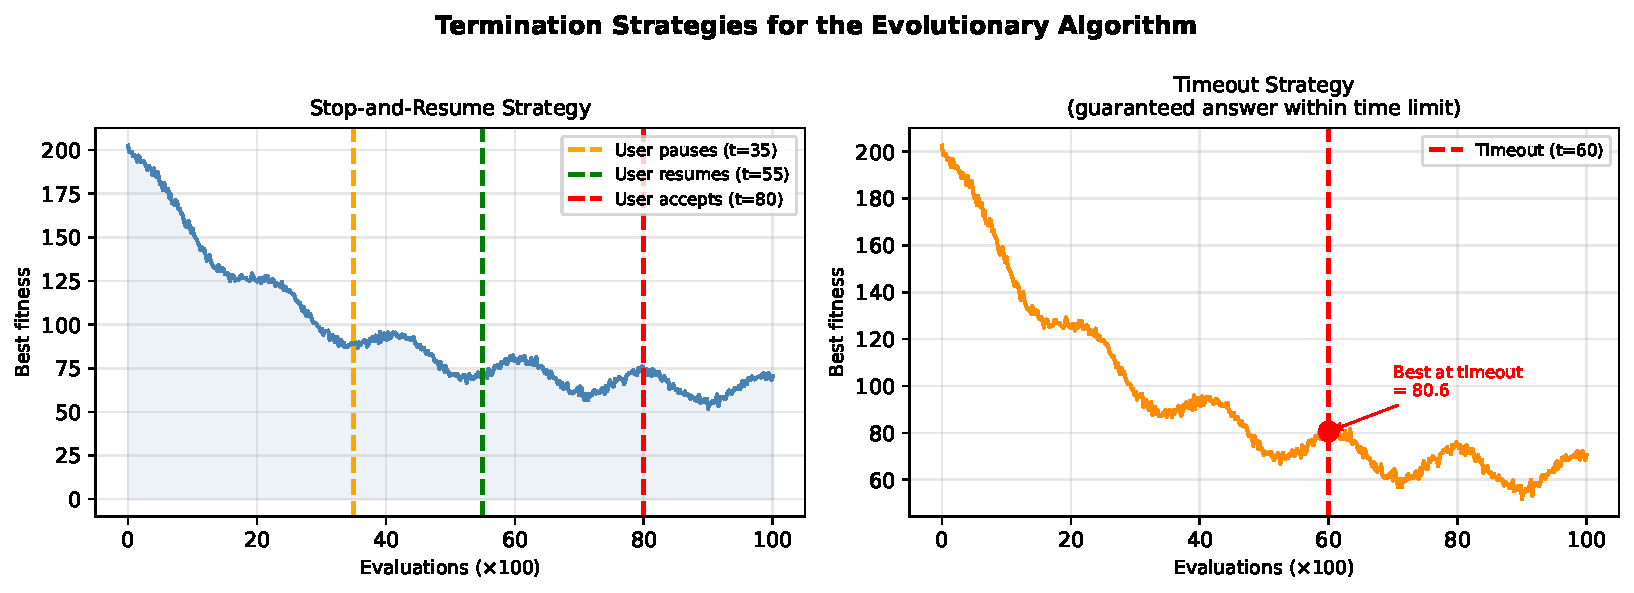
\includegraphics[width=0.82\textwidth]{fig_termination_strategies.pdf}
    \caption{\emph{Left}: stop-and-resume — the user pauses, inspects,
             and then resumes.  \emph{Right}: timeout — the algorithm
             stops automatically at the evaluation budget, guaranteeing
             an answer within a fixed time.  Both panels show that
             fitness improves rapidly early on and then plateaus;
             the termination strategy determines how long we wait
             for that plateau.}
  \end{figure}

  \framebreak

  \begin{block}{Input File Format: The CSV Problem Instance}
    The problem instance is stored as a simple CSV (comma-separated
    values) file, chosen because users can create and edit it with
    any spreadsheet application.  Column A contains a keyword; later
    columns contain values.  Any row whose Column A is empty or
    unrecognised is silently ignored.
  \end{block}

  \begin{center}
    \small
    \begin{tabular}{cllllp{2cm}}
      \toprule
      \textbf{Row} & \textbf{Col A (keyword)} & \textbf{Col B} &
      \textbf{Col C} & \textbf{Col D} & \textbf{Col E} \\
      \midrule
      1  & ref           & Edinburgh Test Problem & & & \\
      2  & capacity      & 30 & & & \\
      3  & mins/delivery & 5 & mins & & \\
      4  & time/round    & 500 & mins & & \\
      5  & mode          & car & & & \\
      6  & commences     & 04/05/2021 09:00 & & & \\
      7  & start         & Napier Univ, EH10 5DT & & & \\
      8  & visit         & 1 & National Museum & Chambers St EH1 1JF & 1 \\
      9  & visit         & 2 & Museum on Mound & The Mound EH1 1YZ & 1 \\
      10 & visit         & 3 & People's Story & Royal Mile EH8 & 1 \\
      \bottomrule
    \end{tabular}
  \end{center}

  Each \textbf{visit} row supplies: a visit number (Col B), a
  human-readable name (Col C), a postal address for geocoding (Col D),
  and the number of bags required (Col E).

\end{frame}

% ─── Java code listing ────────────────────────────────────────
\begin{frame}[fragile]{Java: Main Application (Listing 10.1)}

  The following code (Listing 10.1 from the book) shows the complete
  main application.  The \texttt{FoodFacade} class hides all
  optimisation complexity: the developer needs only four lines of
  logic to load, solve, and save a food-delivery problem.

\begin{lstlisting}[language=Java,
    caption={Listing 10.1: The food application (Java).},
    label={lst:java_main}]
public class FoodDeliveryApp {
  public static void main(String[] args) {
    // Load a problem from a .csv file
    FoodFacade food = loadProblem(new File("./problem.csv"));

    // Run the evolutionary optimiser (all complexity is hidden)
    food.solve();

    // Save the solution in several output formats
    try {
      food.save(SaveTo.CONSOLE);  // print to screen
      food.save(SaveTo.KML);      // Google Earth
      food.save(SaveTo.GPX);      // GPS devices
      food.save(SaveTo.CSV);      // spreadsheet
    } catch (Exception e) {
      e.printStackTrace();
    }
  }
}
\end{lstlisting}

  \begin{exampleblock}{Line-by-Line Explanation}
    \textbf{Line 3} calls \texttt{loadProblem()}, a private helper
    that reads the CSV file and calls the appropriate \texttt{FoodFacade}
    setter methods (e.g.\ \texttt{setCapacity()}, \texttt{addVisit()}).
    \textbf{Line 6} invokes \texttt{solve()}, which runs the entire
    evolutionary algorithm internally — the caller never sees
    population sizes or fitness functions.
    \textbf{Lines 9--12} save the result in four formats: to the
    console for debugging, to KML for Google Earth visualisation, to
    GPX for sat-nav devices, and to CSV for spreadsheet analysis.
  \end{exampleblock}

\end{frame}

\begin{frame}[fragile]{Java: Loading and Parsing the CSV (Listing 10.2)}

  The method \texttt{loadProblem()} reads the CSV file line by line and
  dispatches each line to \texttt{processLine()}, which inspects
  Column A and calls the appropriate \texttt{FoodFacade} setter.
  This design deliberately separates \emph{data parsing} from
  \emph{optimisation logic}: the \texttt{FoodFacade} class has no
  knowledge of the file format.

\begin{lstlisting}[language=Java,
    caption={Listing 10.2: Problem loading and CSV parsing (Java).},
    label={lst:java_load}]
private static FoodFacade loadProblem(File file) {
  // Create a new FoodFacade and populate it from the file
  try {
    FoodFacade food = new FoodFacade();
    Scanner myReader = new Scanner(file);
    while (myReader.hasNextLine()) {
      processLine(food, myReader.nextLine());
    }
    myReader.close();
    return food;
  } catch (FileNotFoundException e) {
    System.out.println("An error occurred.");
    e.printStackTrace();
    return null;
  }
}

private static void processLine(FoodFacade hf, String line) {
  // Process a single line of the .CSV file
  String[] data = line.split(",");
  data[0] = data[0].toLowerCase().trim();
  if (data[0].equals("ref"))        { hf.setReference(data[1]); }
  if (data[0].equals("commences"))  { hf.setStartDateTime(data[1]); }
  if (data[0].equals("start"))      { hf.setStart(data[1]); }
  if (data[0].equals("visit"))      {
    hf.addVisit(data[2], data[3], Integer.parseInt(data[4]), "");
  }
  if (data[0].equals("capacity"))   { hf.setCapacity(Integer.parseInt(data[1])); }
  if (data[0].equals("mins/delivery")) { hf.setMinsDel(Integer.parseInt(data[1])); }
  if (data[0].equals("time/round")) { hf.setMaxMinsRound(Integer.parseInt(data[1])); }
  if (data[0].equals("mode"))       { hf.setRoundMode(data[1]); }
}
\end{lstlisting}

  \begin{exampleblock}{How the Parser Works}
    Each line is split on commas.  The keyword in Column A (lowercased
    and trimmed) is compared to known keywords (\texttt{ref},
    \texttt{commences}, \texttt{start}, \texttt{visit}, etc.).
    For \texttt{visit} rows, \texttt{addVisit()} is called with
    the name, address, demand (number of bags), and an optional
    order string.  Unknown keywords cause no error — they are silently
    skipped.
  \end{exampleblock}

\end{frame}

\begin{frame}[fragile]{Python: Equivalent CSV Loader}

  Below is a Python equivalent of the Java CSV loader above,
  demonstrating how the same logic would be implemented in Python.
  This is useful for understanding the algorithm independent of
  the book's Java implementation.

\begin{lstlisting}[style=python,
    caption={Python equivalent of the food delivery CSV loader.},
    label={lst:python_loader}]
import csv

class FoodFacade:
    """Facade that loads, solves, and saves food delivery problems."""

    def __init__(self):
        self.reference = ""
        self.start_address = ""
        self.start_datetime = ""
        self.capacity = 30         # default: 30 bags
        self.mins_per_delivery = 5 # default: 5 minutes per stop
        self.max_mins_round = 500  # default: 500 minutes per round
        self.mode = "car"
        self.visits = []           # list of (name, address, demand, order)

    def add_visit(self, name, address, demand, order=""):
        self.visits.append({
            "name": name, "address": address,
            "demand": demand, "order": order
        })

    # ... setters for capacity, time limit, etc. ...

    def load_from_csv(self, filepath: str):
        """Load problem definition from a keyword-CSV file."""
        with open(filepath, newline='') as f:
            for row in csv.reader(f):
                if not row or not row[0].strip():
                    continue                   # skip empty rows
                key = row[0].strip().lower()
                if key == "ref":
                    self.reference = row[1]
                elif key == "capacity":
                    self.capacity = int(row[1])
                elif key == "mins/delivery":
                    self.mins_per_delivery = int(row[1])
                elif key == "time/round":
                    self.max_mins_round = int(row[1])
                elif key == "mode":
                    self.mode = row[1]
                elif key == "commences":
                    self.start_datetime = row[1]
                elif key == "start":
                    self.start_address = row[1]
                elif key == "visit":
                    # row: visit, seq, name, address, demand
                    self.add_visit(
                        name=row[2], address=row[3],
                        demand=int(row[4]) if len(row) > 4 else 1
                    )
        return self

    def solve(self):
        """Placeholder: in practice calls the evolutionary algorithm."""
        print(f"Solving for {len(self.visits)} visits, "
              f"capacity={self.capacity}, max_time={self.max_mins_round} min")
        # ... evolutionary algorithm runs here ...


if __name__ == "__main__":
    facade = FoodFacade()
    facade.load_from_csv("problem.csv")
    facade.solve()
\end{lstlisting}

\end{frame}

\begin{frame}[fragile]{Python: Weighted Distance Fitness Function}

  The weighted-distance fitness function is the core of the algorithm.
  This Python implementation computes $WD = \sum_i d_i \times wc_i$
  given a list of pairwise distances and a route (list of customer
  indices).

\begin{lstlisting}[style=python,
    caption={Python: computing the weighted-distance fitness.},
    label={lst:python_wd}]
import numpy as np

def weighted_distance(route: list, dist_matrix: np.ndarray) -> float:
    """
    Compute the weighted-distance fitness of a route.

    Parameters
    ----------
    route       : list of customer indices, e.g. [0, 2, 1, 4, 3]
                  (depot is represented by index -1 or implicitly at
                   the start and end)
    dist_matrix : 2-D numpy array where dist_matrix[i][j] is the
                  distance from location i to location j.
                  Index 0 is assumed to be the depot.

    Returns
    -------
    WD : float -- weighted distance (lower is better)
    """
    n_customers = len(route)
    full_route = [0] + route + [0]   # 0 = depot at start and end
    wd = 0.0

    for i in range(len(full_route) - 1):
        from_idx = full_route[i]
        to_idx   = full_route[i + 1]
        leg_dist = dist_matrix[from_idx][to_idx]

        # wait_count = number of customers NOT yet delivered at leg i
        # (customers delivered so far = i; total = n_customers)
        wait_count = max(0, n_customers - i)

        wd += leg_dist * wait_count

    return wd


# -- Worked example -------------------------------------------
if __name__ == "__main__":
    # 6 locations: depot(0), A(1), B(2), C(3), D(4), E(5)
    # Route: Depot -> A -> B -> C -> D -> E -> Depot
    # Distances: 2, 5, 6, 5, 3, 4 (from textbook example)
    d = np.zeros((6, 6))
    # We'll use a simple sequential distance matrix for illustration
    legs = [(0,1,2),(1,2,5),(2,3,6),(3,4,5),(4,5,3),(5,0,4)]
    for a, b, dist in legs:
        d[a][b] = dist
        d[b][a] = dist  # symmetric

    route = [1, 2, 3, 4, 5]   # A, B, C, D, E
    wd = weighted_distance(route, d)
    print(f"Total distance = {sum(d[a][b] for a,b,_ in legs)}")  # 25
    print(f"Weighted distance WD = {wd}")                         # 86
\end{lstlisting}

  \begin{exampleblock}{Expected Output}
    \texttt{Total distance = 25.0} \\
    \texttt{Weighted distance WD = 86.0} \\
    These match the textbook values exactly, confirming the formula.
  \end{exampleblock}

\end{frame}

% ============================================================
\section{10.4 Results}
% ============================================================

\begin{frame}[allowframebreaks]{10.4 Results: Edinburgh Tourist Attractions Case Study}

  To evaluate the algorithm, the authors created a benchmark problem
  instance based on real Edinburgh tourist attraction addresses.
  This is called the \textbf{Edinburgh Tourist Attractions (ETA)
  instance}.

  \begin{block}{Why a Public Test Instance?}
    The original problem instances used with real clients were
    commercially confidential and could not be published.
    The ETA instance uses publicly available addresses and provides
    a reproducible benchmark for comparing algorithm settings.
    The instances in the study had fewer than 100 deliveries each
    (in practice, fewer than 20 for many real clients).
  \end{block}

  \begin{figure}
    \centering
    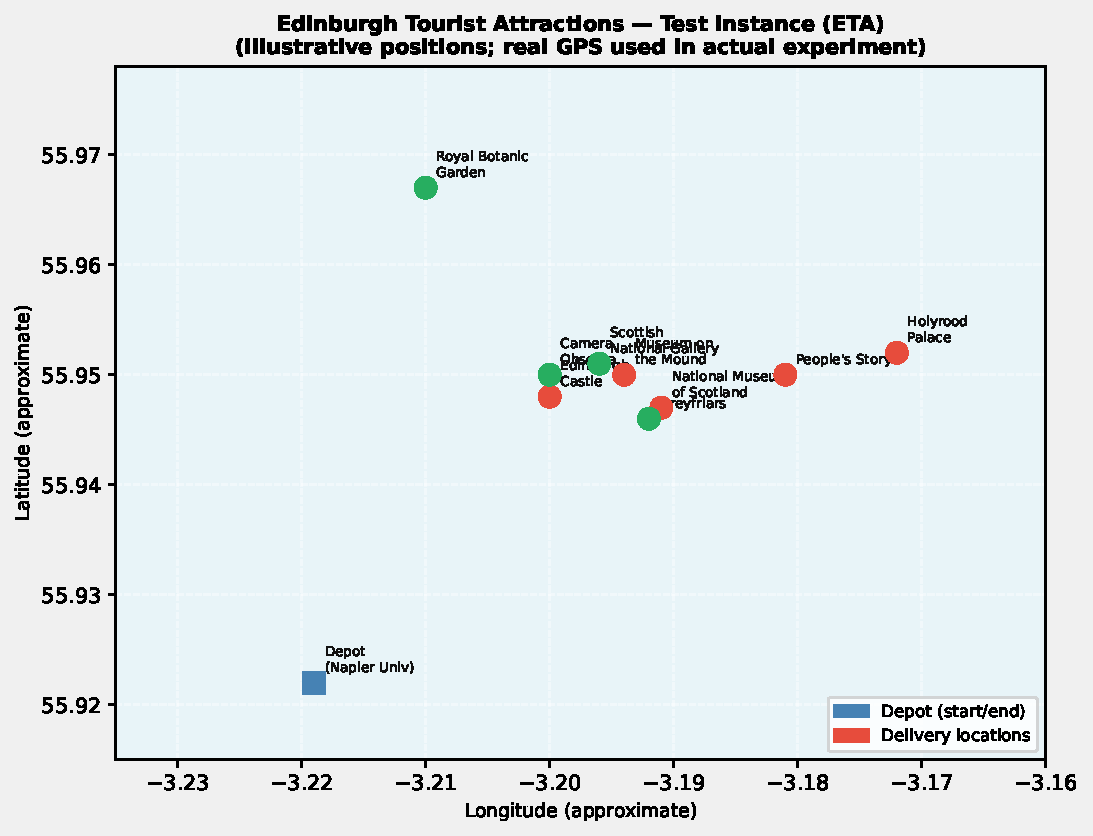
\includegraphics[width=0.65\textwidth]{fig_edinburgh_schematic.pdf}
    \caption{Approximate locations of Edinburgh tourist attractions
             used as delivery stops in the ETA test instance.
             The depot is Edinburgh Napier University (Colinton Road).
             Real experiments used actual GPS coordinates obtained by
             geocoding the postal addresses.}
  \end{figure}

  \framebreak

  \begin{block}{Experimental Design}
    Two sets of experiments were run on the ETA instance, each
    varying one constraint while fixing the others:
    \begin{enumerate}
      \item \textbf{Vehicle capacity experiments (Table 10.3):}
            The maximum transit time was fixed and capacity was varied
            from 5 to 30 bags per round.
      \item \textbf{Transit time experiments (Table 10.4):}
            The vehicle capacity was fixed and the maximum transit
            time was varied from 60 to 500 minutes per round.
    \end{enumerate}
    For each parameter setting, the algorithm was run multiple times
    (multiple independent runs) and the minimum, mean, and maximum
    number of routes was recorded across runs.
  \end{block}

  \framebreak

  \begin{exampleblock}{Interpreting Table 10.3 — Effect of Vehicle Capacity}
    As capacity decreases from 30 to 5 bags, the number of delivery
    routes required increases.  With capacity 30, a single round can
    deliver all bags in just 2 routes on average; with capacity 5, up
    to 6 routes are needed.  This is physically intuitive: a smaller
    vehicle makes more trips.  The spread between minimum and maximum
    routes (``Min Routes'' and ``Max Routes'') also increases at lower
    capacities, reflecting that the algorithm sometimes finds
    better-than-average solutions.
  \end{exampleblock}

  \begin{exampleblock}{Interpreting Table 10.4 — Effect of Transit Time}
    When the maximum transit time per round is tight (e.g., 60 minutes),
    many routes are required because each round can only cover a short
    distance.  As the time limit is relaxed to 500 minutes, fewer routes
    suffice since the vehicle can complete a longer loop in one round.
    As might be expected: \textbf{the more constrained the problem, the
    more routes are required.}
  \end{exampleblock}

  \begin{figure}
    \centering
    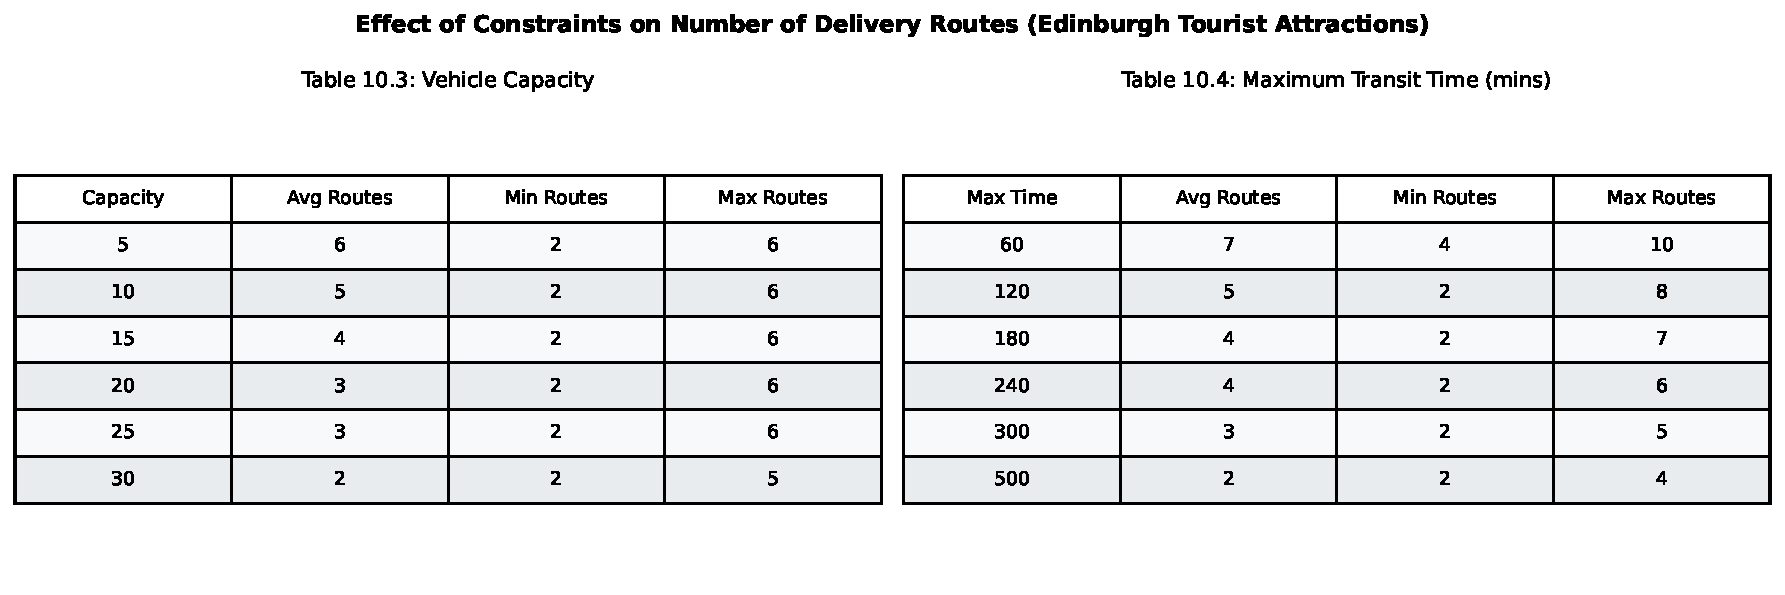
\includegraphics[width=0.85\textwidth]{fig_capacity_table.pdf}
    \caption{\emph{Left (Table 10.3):} effect of vehicle capacity on
             the number of delivery routes (ETA instance).
             \emph{Right (Table 10.4):} effect of maximum transit time
             on the number of routes.
             In both cases, tighter constraints force the algorithm to
             use more routes.}
  \end{figure}

  \framebreak

  \begin{figure}
    \centering
    
\includegraphics[width=0.82\textwidth]{fig_convergence.pdf}
    \caption{\emph{Left:} evolutionary convergence curves comparing
             simple-distance fitness (blue) and weighted-distance
             fitness (orange).  Both converge, but the weighted-distance
             formulation finds solutions that better satisfy user
             expectations about delivery order.
             \emph{Right:} number of routes as a function of vehicle
             capacity, showing the expected monotone decrease as
             capacity increases.}
  \end{figure}

  \begin{alertblock}{Summary of Results}
    The algorithm reliably finds solutions across a wide range of
    capacity and time-limit settings.  Increasing constraints
    (lower capacity or tighter time limits) monotonically increases
    the required number of routes, which is consistent with
    real-world logistics.  The weighted-distance fitness function
    produces routes that better align with customer expectations:
    nearby deliveries happen first, reducing average waiting time.
  \end{alertblock}

\end{frame}

% ============================================================
\section{10.5 Conclusions}
% ============================================================

\begin{frame}[allowframebreaks]{10.5 Conclusions}

  This chapter has demonstrated a complete, deployable solution to the
  food-delivery variant of the Vehicle Routing Problem.  Several
  important lessons emerge.

  \begin{block}{1. Package: Reuse the Algorithm as a Library}
    The evolutionary optimiser is packaged as a \emph{JAR archive}
    (Java ARchive) — a compiled library that any Java application can
    import.  Source code need not be exposed.  This packaging approach
    is widely applicable: algorithm developers can ship their code as
    a library, and application developers integrate it without
    understanding the internals.  Python equivalents include
    distributing code as a wheel (\texttt{.whl}) package on PyPI.
  \end{block}

  \begin{block}{2. Configure: Manage Execution Time}
    Waiting for an algorithm to finish is unacceptable in interactive
    applications.  Providing configurable timeout values and
    stop-and-resume controls ensures that the user always receives
    an answer within a predictable time.  The specific timeout values
    (and other parameters such as population size and mutation rate)
    are stored in a properties file, so a system administrator can tune
    them without modifying or recompiling the application.
  \end{block}

  \begin{block}{3. Multiple Runs: Compensate for Randomness}
    Because evolutionary algorithms are stochastic (they use random
    numbers), a single run may find a solution that is better or worse
    than typical.  Running the algorithm several times and presenting
    the best result across runs dramatically increases the probability
    of finding a high-quality solution.  The multiple-run strategy is
    especially effective when combined with a fixed timeout: each
    run is allocated a fraction of the total budget.
  \end{block}

  \begin{block}{4. Fitness Function: Weighted Distance over Simple Distance}
    Using \emph{weighted distance} as the fitness function rewards
    the algorithm for making early deliveries.  Feedback from real
    users confirmed that this is indeed what they expected: customers
    who receive their delivery early in the route are more satisfied,
    even if the total route length is slightly longer.
  \end{block}

  \framebreak

  \begin{alertblock}{Broader Takeaway: Algorithm + Engineering}
    A powerful algorithm alone is not sufficient for real-world impact.
    Successful deployment requires:
    \begin{itemize}
      \item A \textbf{well-designed fitness function} that captures true
            user preferences (not just a proxy like total distance).
      \item A \textbf{clean software architecture} (Facade pattern, layered
            design) that separates the optimiser from the application.
      \item \textbf{Practical termination strategies} that guarantee
            timely answers to users.
      \item A \textbf{configurable interface} so that domain experts
            (not just algorithm researchers) can tune and deploy the system.
    \end{itemize}
  \end{alertblock}

  \begin{exampleblock}{Food Delivery as a Template}
    The architecture described in this chapter — base library $\to$
    domain-specific subclasses $\to$ Facade API — is reused in the
    following two chapters for letter and parcel delivery.
    The same pattern can be applied to any combinatorial optimisation
    problem: vehicle routing, staff scheduling, facility location, etc.
  \end{exampleblock}

\end{frame}

% ============================================================
%  Summary slide
% ============================================================
\begin{frame}{Chapter 10 Summary}

  \begin{columns}[T]
    \begin{column}{0.48\textwidth}
      \begin{block}{What We Covered}
        \begin{itemize}
          \item Food delivery as a constrained VRP: capacity $Q$,
                max transit time, min delivery time
          \item Weighted distance $WD = \sum d_i \times wc_i$
                as a user-aligned fitness function
          \item Three-layer software architecture with Facade pattern
          \item CSV input format and Java/Python parser
          \item Stop-and-Resume vs.\ Timeout termination
          \item ETA case study: effect of capacity and time constraints
        \end{itemize}
      \end{block}
    \end{column}
    \begin{column}{0.48\textwidth}
      \begin{block}{Key Formulas}
        Simple distance:
        \[F_{\text{dist}} = \sum_{i=1}^{n} d_i\]
        Weighted distance:
        \[WD = \sum_{i=1}^{n} d_i \times wc_i\]
        where $wc_i = (\text{customers left at leg } i)$.
        \\[6pt]
        For 5 customers, route Dep$\to$A$\to$B$\to$C$\to$D$\to$E$\to$Dep:\\
        $F_{\text{dist}} = 25$, $WD = 86$.
      \end{block}

      \begin{alertblock}{Core Principle}
        Design the \textbf{fitness function} to reward the behaviour
        you actually want — not just the easiest thing to measure.
      \end{alertblock}
    \end{column}
  \end{columns}

\end{frame}

% ============================================================
%  Reference slide
% ============================================================
\begin{frame}{References}
  \begin{itemize}
    \item \textbf{Amos, D., Calinescu, R., et al.\ (2022).}
          \textit{Nature Inspired Optimisation for Delivery Problems}.
          Springer, Chapter 10: Delivering Food, pp.\ 209--221.
    \item \textbf{Gamma, E., Helm, R., Johnson, R., \& Vlissides, J.\ (1994).}
          \textit{Design Patterns: Elements of Reusable Object-Oriented
          Software}.  Addison-Wesley.
          [Facade pattern, p.\ 185.]
    \item \textbf{Clarke, G., \& Wright, J.W.\ (1964).}
          Scheduling of vehicles from a central depot to a number of
          delivery points.
          \textit{Operations Research}, 12(4), 568--581.
          [Foundational VRP paper.]
    \item \textbf{Toth, P., \& Vigo, D.\ (Eds.)\ (2002).}
          \textit{The Vehicle Routing Problem}.
          SIAM, Philadelphia.
  \end{itemize}
\end{frame}

\end{document}
